\documentclass[a4paper, 12pt, twoside]{report}

% This can be used if you want to increase the spacing between lines to 1.5x
%\linespread{1.5}

%General packages

% Uncomment the following line for preparing the final hardcopy (and comment out the next one)
%\usepackage[a4paper,left=40mm,right=20mm,top=30mm,bottom=20mm]{geometry}
% Use this for your draft (easier to read). Don't forget to manually check
% everything when you switch to final hardcopy geometry (see above)
\usepackage[a4paper,left=20mm,right=20mm,top=30mm,bottom=20mm]{geometry}

\usepackage[utf8]{inputenc}
\usepackage{graphicx}
\usepackage{gensymb}
\usepackage{textcomp}
\usepackage{amsfonts}
\usepackage{appendix}
\usepackage{listings}
%\lstset{breaklines=true}
%\DeclareGraphicsExtensions{.pdf,.jpeg,.png}
\usepackage{amsmath}
\usepackage{amssymb}
\usepackage{algpseudocode}
\usepackage{algorithm}
%\usepackage{array}
\usepackage{subfig}
%\usepackage{captcont}
\usepackage{booktabs}
\usepackage[hyphens]{url}
\usepackage{multirow}
\usepackage{parskip}
%\usepackage{cite}
\usepackage[table]{xcolor}
\usepackage{hyperref}
\usepackage{amsfonts}
\usepackage{amsthm}
\usepackage{mathrsfs}

\newtheorem*{theorem*}{Theorem}
\newtheorem{theorem}{Theorem}[section]

\theoremstyle{definition}
\newtheorem{definition}{Definition}[section]
\newtheorem{exmp}{Example}[section]

\theoremstyle{remark}
\newtheorem*{rem}{Remark}

\def\NN{\ensuremath{\mathbb{N}}}
\def\N{\ensuremath{\mathbb{N}}}
\def\ZZ{\ensuremath{\mathbb{Z}}}
\def\Z{\ensuremath{\mathbb{Z}}}
\def\QQ{\ensuremath{\mathbb{Q}}}
\def\Q{\ensuremath{\mathbb{Q}}}
\def\RR{\ensuremath{\mathbb{R}}}
\def\R{\ensuremath{\mathbb{R}}}
\def\CC{\ensuremath{\mathbb{C}}}
\def\FF{\ensuremath{\mathbb{F}}}
\def\Pr{\ensuremath{\mbox{Pr}}}
%\newsavebox{\imagebox}

%Formatting for headers and footers
\usepackage{fancyhdr}
\pagestyle{fancy}
\fancyhead{}
%\fancyhead[RO,LE]{Monolithic Nanocomposite Detector for LaBrAT-PET}
\renewcommand{\headrulewidth}{0pt}
\fancyfoot{}
\fancyfoot[LE,RO]{\thepage}
%\fancyfoot[LO,RE]{Student Name}

%Bibliography settings
\usepackage[backend=biber,sorting=none,style=ieee]{biblatex}
\addbibresource{library.bib}

%Link to graphics folder
\graphicspath{{figures/}}

% Set your thesis title and author details here
\title{Thesis Title}
\author{Author Name}
\date{\today}

\begin{document}

\begin{titlepage}
\begin{center}
%\vspace*{1cm}

\Huge
\makeatletter
\textbf{\@title}

\Large

\vspace{3.cm}

by \textbf{\@author{}}

\vfill
\large
Thesis submitted in fulfilment of the requirements for the degree of\\
\textit{Bachelor of Science}\\
under the supervision of Tristram Bogart\\
\vfill
\large
Department of Mathematics\\
Faculty of Science\\
Universidad de los Andes\\

\today
\makeatother

\end{center}
\end{titlepage}


\chapter*{Certificate of Authorship / Originality}

\makeatletter

I, \@author{}, declare that this thesis is submitted in fulfilment of the requirements for the award of Doctor of Philosophy, in the School of Electrical and Data Engineering at the University of Technology Sydney.
\makeatother

\vspace{6pt}

\noindent This thesis is wholly my own work unless otherwise referenced or acknowledged. In addition, I certify that all information sources and literature used are indicated in the thesis. This document has not been submitted for qualifications at any other academic institution.

% If applicable, the above statement must be replaced with the collaborative doctoral degree statement (see below).

% If applicable, the Indigenous Cultural and Intellectual Property (ICIP) statement must be added (see below).

\vspace{6pt}

\noindent This research is supported by the Australian Government Research Training Program.

% If you have a top-up or other scholarship, please modify this.

\vspace{1cm}

\begin{tabular}{m{3cm}m{7cm}}
Signature: &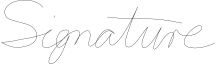
\includegraphics[width=6cm]{example_signature}\\

Date:	&\today\\
\end{tabular}
\vspace{6pt}

\makeatletter

% Can also use a copyright statement as below
%\hfill $\copyright$ Copyright \today{} \@author{}

\makeatother


\pagenumbering{roman}

\chapter*{Abstract}

This is the text of the abstract, providing a brief summary of the context, research problem, main contributions and conclusions of this work.


\chapter*{Dedication}

To my parents, for always loving and supporting me. 
To Mrtn Prd Grr


\chapter*{Acknowledgements}


I would like to thank Tristram Bogart for being an amazing advisor and for his guidance and support. Furthermore, a special thanks to John Goodrick for introducing me to the theory of computation and for his help and advice. In addition, a big thank you goes to the Polymath Jr. program, especially to Christopher O'Neill for introducing me to numerical semigroups, and to Johanna Franklin, for being cool mentors and for their support in guiding me into the world of research. I am also grateful to Alexander Getmanenko for his insightful seminars and book picks, to Adolfo Quiroz for his fun and engaging classes, as well as his advice, and to Monika Winklmeier, Ramiro de la Vega, Mauricio Velasco and Mauricio Junca for their exceptional teaching. Finally, I would like to extend my gratitude to my friends, who have made my undergraduate experience both fun and memorable. \par


{
\makeatletter
\vspace{1cm}
\raggedleft
\@author{}\\
\today{}\\
Bogotá, Colombia\\
\raggedright
\makeatother
}


\tableofcontents
\listoffigures
\listoftables

\pagenumbering{arabic}

% Add additional chapters as required
\chapter{Introduction}\label{chap:intro}


The Probabilistic Method is a powerful tool, with applications in Combinatorics, Graph Theory, Number Theory and Computer Science. It is a nonconstructive method that proves the existence of an object with a certain property, usually a graph, by showing that the probability that a randomly chosen object has that property is greater than zero. In this thesis, we will apply the probabilistic method to numerical semigroups. \par

A numerical semigroup is a subset of $\NN$ that is closed under addition (Definition \ref{def:smgps}). These objects are studied in the context of commutative algebra and algebraic geometry, and they have applications in integer programming, coding theory and cryptography \cite{assi2020numerical}. There are numerical invariants that are used to study numerical semigroups, such as the embedding dimension, the genus and the Frobenius number (Definitions \ref{def:smgps:embedding_dim}, \ref{def:smgps:genus} and \ref{def:smgps:frobeniusnum}). For example, the Frobenius number is defined as the maximum of the complement of the numerical semigroup over the integers. \par

The Erdös-Rényi (ER) model is a commonly used model of random graphs, where each edge is chosen with probability $p$, independently of the other edges (Definition \ref{def:probmet:ermodel}). In contrast to graphs, the study of random models of numerical semigroups requires the use of number theory tools due to their algebraic nature. This thesis investigates the average behavior of random numerical semigroup invariants using a probabilistic model similar to the ER model (Definition \ref{def:randnumsems:ermodel}).


Our central result is Theorem \ref{thm:main}, which is similar to Theorem \ref{thm:ermodel}, the main result of 
\begin{itemize}
    \item \fullcite{de2018random}.
\end{itemize}
Theorem \ref{thm:ermodel} describes the behavior of the expected embedding dimension, genus, and Frobenius number of a random numerical semigroup, depending on the parameters of the model. It gives an explicit bound of the expected value of these invariants. On the other hand, Theorem \ref{thm:main} describes the behavior of the invariants almost surely, that is, with probability that tends to one as the parameters of the model converge to certain values. Our proof is more elementary and provides asymptotically tighter bounds on the behaviour of these invariants. 

We used experiments to study the behavior of ER-type random numerical semigroups, which led to the proof of Theorem \ref{thm:main}. For our experiments, we used \verb|numsgps-sage| \cite[O'Neill]{oneill2018}\cite[Delgado]{delgado2015numericalsgps} and for visualizations we used \verb|IntPic| \cite[Delgado]{delgado2013intpic}. We also implemented our own publicly available repository \verb|randnumsgps| \cite{morales2023} for generating and visualizing random numerical semigroups in Python.\par

The structure of the thesis is as follows:

\begin{itemize}
    \item Chapter \ref{chap:probmet} discusses the Probabilistic Method, based on the work of Noga Alon and Joel H. Spencer.
    \item Chapter \ref{chap:numsems} focuses on numerical semigroups, providing definitions, examples, and results necessary for understanding their structure.
    \item Chapter \ref{chap:randnumsems} introduces three models of random numerical semigroups, including our newly proposed model. We also present recent results in the field, including Theorem \ref{thm:ermodel}. 
    \item Chapter \ref{chap:experiments} details the algorithms and experiments conducted.
    \item Chapter \ref{chap:results} presents the main results, including the proof of Theorem \ref{thm:main}, its implications and its relation with Theorem \ref{thm:ermodel}.
\end{itemize}

To sum up, we provide a detailed study of random numerical semigroups using probabilistic models, experimental data and software tools.\par


Test \cite{thesis_template}

\chapter{Literature Review}\label{chap:litrev}

\section{Introduction}\label{sec:litrev:intro}

Some contextural overview of what we are going to discuss.

Section \ref{sec:litrev:theme1} discusses Theme 1. Section \ref{sec:litrev:theme2} discusses Theme 2....

\section{Theme 1}\label{sec:litrev:theme1}

\subsection{Subtopic A}\label{sec:litrev:theme1:A}

\subsection{Subtopic B}\label{sec:litrev:theme1:B}

\subsection{Subtopic C}\label{sec:litrev:theme1:C}

\section{Theme 2}\label{sec:litrev:theme2}

Etc. etc.

\section{Conclusion}\label{sec:litrev:conclusion}


% All contribution chapters should follow a similar structure, with a
% mini-introduction and overview at the beginning and a conclusion at the
% end bookmarking a structured presentation of the contribution. This can be
% largely based on your publications.

\chapter{Contribution 1}\label{chap:contrib1}

\section{Introduction}

In this Chapter, XXX is presented. Note: to cross-reference to other parts of the document you do so like this - see Section \ref{sec:contrib2:theme1:B}.

Section \ref{sec:contrib1:theme1} discusses Theme 1. Section \ref{sec:contrib1:theme2} discusses Theme 2....

\section{Theme 1}\label{sec:contrib1:theme1}

\begin{figure}
\centering
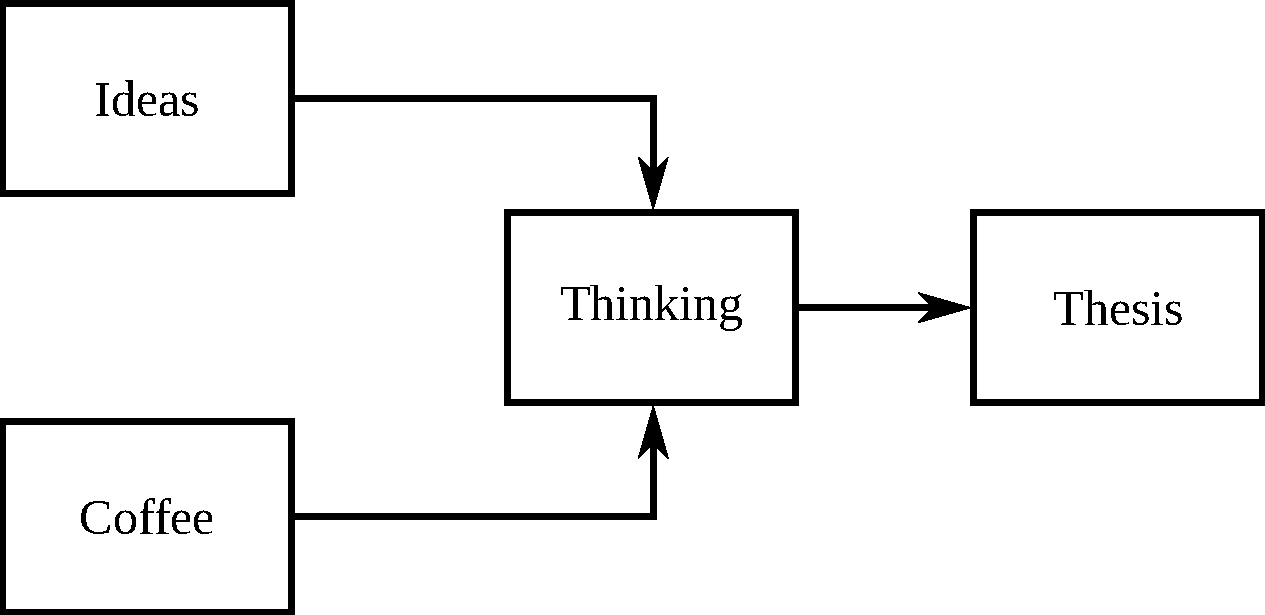
\includegraphics[width=0.8\textwidth]{sample_wide_figure}
\caption{This the approximate process for producing a Thesis. It typically takes 3-4 years.}
\label{fig:phd_life}
\end{figure}

\figurename{} \ref{fig:phd_life} illustrates the key elements of Thesis synthesis. \LaTeX{} will tend to place figures where it wants (they `float' - generally they should be at the top or bottom of a page); you can override the default behaviour if you want, but you probably don't want to bother doing that until after your content is pretty much done. Instead, keep the figures as close as possible to the text; you can tweak this afterwards if you want by adding an option:

\begin{verbatim}
\begin{figure}[htb]
\end{verbatim}

This says put it here, if you can, otherwise at the top, or otherwise at the bottom. BUT I strongly suggest not using {\bf h} as it looks terrible.

Maybe you need an inline URL at this point: Here's one! \url{https://en.wikibooks.org/wiki/LaTeX}.

Mathematics can be inline, for example $x = \int_0^\infty y^2 dy$, or can be in display mode, as shown in \eqref{eqn:example}:

\begin{equation}
\label{eqn:example}
F(x,y,z) = \sqrt{x^{y^z}}
\end{equation}

You probably want to show some of your results in a table, such as \tablename{} \ref{tab:example}.

% Table environment. This is the most difficult thing to get right in LaTeX if you go beyond a simple table like that shown below. Refer to the LaTeX Wikibook for lots of info about creating LaTeX tables (see the toplevel README.md).
\begin{table*}
\centering
\caption{Table captions normally go at the top.}
\label{tab:example}
% Don't leave blank lines in the middle of a floating environment such as table or figure!
% This bit describes how the columns are organised. l, r, c for left, right, centre-justified; p{1cm} or p{0.2\textwidth} for left-justified with fixed width. This is usually best.
\begin{tabular}{p{0.2\textwidth}p{0.3\textwidth}p{0.3\textwidth}}
\toprule
{\bf Left column}	&{\bf $\mu$}	&{\bf $\sigma$}\\
\midrule
Item 1				&0.3			&0.5\\
Item 2				&0.9			&0.4\\
\bottomrule
\end{tabular}
\end{table*}

\begin{figure}
\centering
\subfloat[Confusion]{
	
\includegraphics[height=0.3\textwidth]{confusion}
	\label{fig:confusion}
}
\subfloat[Work]{
	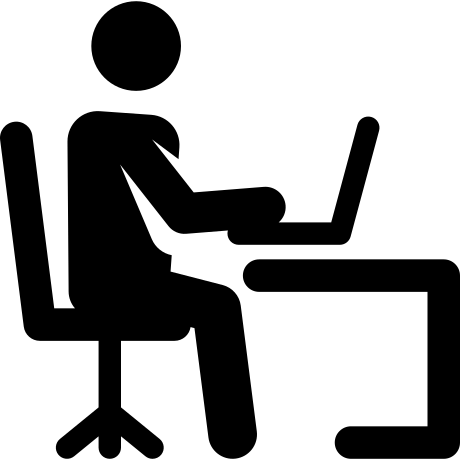
\includegraphics[height=0.3\textwidth]{work}
	\label{fig:work}
}
\subfloat[Exhaustion]{
        
\includegraphics[height=0.3\textwidth]{exhaustion}
        \label{fig:exhaustion}
}
\caption{The stages of the creative process.}
\label{fig:creative_process}
\end{figure}

The basic creative process is shown in \figurename{} \ref{fig:creative_process}. Specifically, \figurename{} \ref{fig:confusion} shows the first step, while \figurename{} \ref{fig:work} and \ref{fig:exhaustion} show the remaining key steps of the procedure.

\subsection{Subtopic A}\label{sec:contrib1:theme1:A}

Algorithm \ref{alg:cap} shows a classical algorithm typeset in \LaTeX{}. This is also a float.

\begin{algorithm}
\caption{An algorithm with caption}\label{alg:cap}
\begin{algorithmic}
\Require $n \geq 0$
\Ensure $y = x^n$
\State $y \gets 1$
\State $X \gets x$
\State $N \gets n$
\While{$N \neq 0$}
\If{$N$ is even}
    \State $X \gets X \times X$
    \State $N \gets \frac{N}{2}$  \Comment{This is a comment}
\ElsIf{$N$ is odd}
    \State $y \gets y \times X$
    \State $N \gets N - 1$
\EndIf
\EndWhile
\end{algorithmic}
\end{algorithm}

\subsection{Subtopic B}\label{sec:contrib1:theme1:B}

\subsection{Subtopic C}\label{sec:contrib1:theme1:C}

\section{Theme 2}\label{sec:contrib1:theme2}

Etc. etc.

\section{Introduction}

\section{Kahn-Kalai Conjecture}

\subsection{Thresholds}

Let $n \in \N$ and $0 \leq p \leq 1$. The random graph $G(n, p)$ is a probability space over the set of graphs on $n$ labeled vertices determined by
\[\Pr[\{i, j\} \in G] = p\] 
with these events mutually independent \cite{alon2016probabilistic}. Given a graph theoretic property $A$, there is a probability that $G(n, p)$ satisfies $A$, which we write as $\Pr[G(n, p) \vDash A]$. 

\begin{definition}
    $r(n)$ is a threshold function for a graph theoretic property $A$ if 
    \begin{enumerate}
        \item When \(p(n) \in o(r(n)), \; \lim_{n \to \infty} \Pr[G(n, p(n)) \vDash A] = 0,\)
        \item When \(r(n) \in o(p(n)), \;  \lim_{n \to \infty} \Pr[G(n, p(n)) \vDash A] = 1,\) 
    \end{enumerate}
    or vice versa. \cite{alon2016probabilistic}
\end{definition}

We give an example of a threshold function which illustrates a common method for proving that a function is a threshold. \par

\subsubsection{Threshold function for having isolated vertices}

Let $G$ be a graph on $n$ labeled vertices. An isolated vertex of $G$ is a vertex which does not belong to any of the edges of $G$. Let $A$ be the property that $G$ contains an isolated vertex. We will prove that $\displaystyle{r(n) = \frac{\ln n}{n}}$ is a threshold for $A$. \par

For each vertex $i$ in $G$ define the variable 

\[X_i = 
\left\{
	\begin{array}{ll}
		1  & \mbox{if } i \text{ is an isolated vertex,} \\
		0 & \mbox{if } i \text{ is not an isolated vertex.}
	\end{array}
\right.
\]

Now, the probability that a vertex $i$ is isolated is $(1 - p)^{n - 1}$ since it is the probability that none of the other $n - 1$ vertices is connected to $i$. Let $X = \sum_{i = 1}^n X_i$, then the expected number of isolated vertices is
 \[E[X] = \sum_{i = 1}^{n} E[X_i] = \sum_{i = 1}^{n} \Pr[X_i] = n(1 - p)^{n - 1}.\]

Let $\displaystyle{p = k\frac{\ln n}{n}}$ for $k \in \R_{>0}$. Then
\begin{align*}
    \lim_{n \to \infty} E[X] &= \lim_{n \to \infty} n\left(1 - k\frac{\ln n}{n}\right)^{n - 1} \\
    &= ne^{-k\ln n} = n^{1 - k}.
\end{align*}

Therefore, $\lim_{n \to \infty} E[X] = 0$ if $k > 1$. Since \(E[X] \geq \Pr[X > 0],\) we conclude that \[\lim_{n \to \infty} \Pr[G(n, p) \vDash A] =  \lim_{n \to \infty} \Pr[X > 0] = 0.\] \par
Now, for $k < 1$, the fact that $\lim_{n \to \infty} E[X] = \infty$ is not enough to conclude that \(\lim_{n \to \infty} \Pr[G(n, p) \vDash A] = 1\). We have to use the second moment method. \par

\begin{theorem*}
    If $E[X] \to \infty$ and $\text{Var}[X] = o(E[X]^2)$, then $\lim_{n \to \infty} \Pr[X > 0] = 1$. \cite{alon2016probabilistic}
\end{theorem*}

\textbf{Proof. } We will prove that, in this case, $Var[X] = o(E[X]^2)$. First, 
\begin{align*}
    \sum_{i \neq j}E[X_iX_j] &= \sum_{i \neq j} \Pr[X_i = X_j = 1] \\
    &= n(n - 1)(1 - p)^{n -1}(1 - p)^{n - 2} \\ &= n(n - 1)(1 - p)^{2n - 3},
\end{align*}

for if $i$ is an isolated vertex, then there is no edge between $i$ and $j$ so we only have to account for the remaining $n - 2$ edges that contain $j$.  \par

Thus, since $\sum_{i = 1}^{n}E[X_i^2] =  \sum_{i = 1}^n E[X_i] = E[X]$ and $\lim_{n \to \infty} p = 0$,

\begin{align*}
    \lim_{n \to \infty} \frac{\text{Var}[X]}{E[X]^2} &= 
    \lim_{n \to \infty}\frac{E(X^2) - E[X]^2}{E[X]^2} = \lim_{n \to \infty} \frac{\sum_{i = 1}^n E[X_i^2] + \sum_{i \neq j}E[X_iX_j]}{E[X]^2} - 1 \\ &= 0 + \lim_{n \to \infty} \frac{ n(n - 1)(1 - p)^{2n - 3}}{n^2(1 - p)^{2n - 2}} - 1= \lim_{n \to \infty} \frac{1}{1 - p} - 1 = 0.\\
\end{align*} \par
We conclude that $\text{Var}[X] \in o(E[X]^2)$ and so, if $k < 1$, \[\lim_{n \to \infty} \Pr[G(n, p) \vDash A] = \lim_{n \to \infty} \Pr[X > 0] = 1.\] Therefore, $r(n) = \frac{\ln n}{n}$ is a threshold function for property $A$.

\subsection{The expectation threshold}

Let $X$ be a set and $p \in [0, 1]$. For $A \subset X$, let $P(A) = p^{|A|}(1 - p)^{|X \setminus A|}$. A class $\mathcal{F}$ of subsets of $X$ is increasing if for $A \in \mathcal{F}$, $A \subset B$ implies $B \in \mathcal{F}$. If $\mathcal{F} \neq \emptyset$,  $P(\mathcal{F}) = \sum_{A \in \mathcal{F}} P(A)$ is a strictly increasing function of $p$.
 
\textbf{TODO} Define increasing class and general definition of threshold \cite{park2022proof} 

\noindent \textbf{TODO} Define expectation threshold and show inequalities. \cite{frankston2021thresholds}

\begin{theorem}[Park Theorem \cite{park2022proof}, originally Kahn-Kalai Conjecture]
\textbf{TODO}
\end{theorem}

\textbf{TODO} How to prove something is p-small

\subsubsection{An application of the Park Theorem}

\noindent \textbf{TODO} Prove the threshold for perfect matchings for $G(n, p)$

\section{Numerical Semigroups}

A \textit{numerical semigroup} is a subset $S \subset \NN_{0}$ which is closed under addition, i.e. $a, b \in S$ implies $a + b \in S$. For instance, $\NN_0$, $\NN_0 \setminus \{0\}$, $2\NN_0$ are all numerical semigroups, but $\NN_0 \setminus \{2\}$ is not. Some literature requires that a semigroup has a finite complement in $\Z_{\geq 0}$ \cite{chapman2020beyond}, but we prefer the more general definition. 

\begin{exmp} \textbf{TODO}
    McNugget Semigroup
\end{exmp}

As seen in the previous example, we can describe a numerical semigroup with a set of \textit{generators}: 
\[S = \langle a_1, ..., a_n \rangle := \left\{\sum_{i = 1}^n k_ia_i: k_1,...,k_n \in \NN_0\right\}.\] \textbf{TODO} give some examples.

The \textit{Frobenius number} $F(S)$ of a numerical semigroup $S = \langle a_1, ..., a_n \rangle$ is defined as the largest integer divisible by $d(S) := \gcd(a_1, ..., a_n)$ which does not belong to $S$. In other terms, 
\[F(S) = \max (d \ZZ \setminus S).\]

\section{Probability Spaces over Numerical Semigroups}

We generate a random numerical semigroup with a model similar to the Ërdos-Renyi model for random graphs. 

\begin{definition}
    For $p \in [0, 1]$ and $M \in \NN$, a random numerical semigroup $S(M, p)$ is a probability space over the set of semigroups $S = \langle\mathcal{A}\rangle$ with $\mathcal{A} \subset \{1,...,M\}$, determined by
    \[\Pr[n \in \mathcal{A}] = p,\]
    with these events mutually independent.
\end{definition}


\section{Expected Frobenius Number}

We prove a Theorem found in \cite{de2017random} without the use of the simplicial complex. 

\begin{theorem}
    Let $S \sim S(M, p)$, where $p = p(M)$ is a monotone decreasing function of M. If $\frac{1}{M} \ll p \ll 1$, then $S$ is cofinite, i.e., the set of gaps is finite, a.a.s and 
\[\lim_{M \to \infty} E[e(S)] = \lim_{M \to \infty} E[g(S)] = \lim_{M \to \infty} E[F(S)] = \infty.\]
\end{theorem}

\textbf{Proof. } Let $X := \min(S \setminus \{0\})$ be a random variable. Then, for $0 < n \leq M$,
\begin{align*}
    \Pr[X = n] = p(1 - p)^{n - 1}, 
\end{align*}
and so 
\begin{align*}
    E[X] &= \sum_{n = 0}^{\infty} n\Pr[X = n] =
    \sum_{n = 0}^{M} np(1 - p)^{n - 1} = p\frac{d}{dp}\left[-\sum_{n = 0}^{M}(1 - p)^n\right]\\
    &=p\frac{d}{dp} \frac{(1 - p)^{M + 1} - 1}{p} = p\frac{1 - (1 - p)^{M + 1} - (M  + 1)(1 - p)^Mp}{p^2} \\
    &= \frac{1 - (1 - p)^{M} - M(1 - p)^Mp}{p} \geq \frac{1 - e^{-Mp} - Mpe^{-Mp}}{p}. \\
\end{align*}
Thus, since $\lim_{M \to \infty} Mp = \infty$, then $\lim_{M \to \infty }Mpe^{-Mp} = \lim_{M \to \infty} e^{-Mp} = 0$, which implies that
\[\lim _{M \to \infty} E[X] = \lim_{M \to \infty} \frac{1 - e^{-Mp} - Mpe^{-Mp}}{p} = \infty.\]
Also, note that if $p = \frac{c}{M}$, $c \in \mathbb{R_+}$ ($0 < e^{-c} + ce^{-c} < 1$),
\[\lim _{M \to \infty} E[X] = \lim_{M \to \infty} \frac{1 - e^{-c} - ce^{-c}}{p} = \infty.\]
\newpage
\textbf{Proof. }
Fix $a \in \NN$ such that $a > 11$ and let $A = \{1, \ldots, \lfloor\frac{a}{p}\rfloor\}$. Since   $\frac{1}{M} \ll p$, we have that $\lfloor\frac{a}{p}\rfloor \leq M$ for large enough $M$. Consider the following events:
\begin{itemize}
    \item $E_1$: No generator selected is less than $\frac{1}{ap}$.  \par
    Let $X_1$ be the number of generators selected from $\{1,\ldots,\lfloor\frac{1}{ap}\rfloor\}$. Then 
    \[\Pr[\overline{E_1}] = \Pr[X_1 > 0] \leq E[X_1] \leq p \cdot \frac{1}{ap} = \frac{1}{a}.\]

    \item $E_2:$ At most $\frac{3a}{2}$ generators are selected from $A$.\par 
    Let $X_2$ be the number of generators selected in $A$, then $X_2$ is a binomial random variable with $n = \frac{a}{p}$ and we can use the bound (Feller \textcolor{blue}{I can add this to the appendix})

    \[\Pr[\overline{E_2}] = \Pr\left[X_2 > \frac{3a}{2}\right] \leq  \frac{\frac{3a}{2}(1 - p)}{(\frac{3a}{2} - a)^2} \leq \frac{6}{a}.\]

    Also, note that by the union bound \[\Pr[E_1\land E_2] \leq 1 - \frac{1}{a} - \frac{6}{a} = 1 - \frac{7}{a}.\]  

    \item $E_3:$ At least $\frac{a}{2}$ generators are selected from $A$. \par 
    Similarly, we can use the bound for the other tail of the distribution so that 
    \[\Pr[ \overline{E_3}] = \Pr\left[X_2 < \frac{a}{2}\right] \leq  \frac{(n - \frac{a}{2})p}{(np - \frac{a}{2})^2} = \frac{a - (\frac{a}{2})p}{(\frac{a}{2})^2} \leq \frac{4}{a}.\]
    
    \item $E_4:$ The generators selected from $A$ are minimal.\par 
    Let $Y_{(1)}, Y_{(2)}, \ldots, Y_{(k)}$ denote the first $k$ generators selected in $A$. Assume $E_1$ and $E_2$. We have that $E_1$ implies $Y_{(1)} \geq \frac{1}{ap}$ and $E_2$ implies $k \leq \frac{3a}{2}$. \par
    First we bound for the probability that, given $E_1$ and $E_2$, $b \in A$ is selected as a generator. By conditional probability 
    \begin{align*}
        \Pr[b \text{ is selected}] &= \Pr[b \text{ is selected}|E_1 \land E_2]\Pr[E_1 \land E_2]  \\
        &+  \Pr[b \text{ is selected}|\overline{E_1 \land E_2}]\Pr[\overline{E_1 \land E_2}],
    \end{align*}
    and so
    \[\Pr[b \text{ is selected}|E_1 \land E_2] \leq \frac{\Pr[b \text{ is selected}]}{\Pr[E_1 \land E_2]} \leq  \frac{p}{1 - \frac{7}{a}}.  \] 
    Now, note that $Y_{(2)}$ is not minimal if a multiple of $Y_{(1)}$ is selected in $A$. Thus, if we fix $Y_{(1)} = y_1 \geq \frac{1}{ap}$, $Y_{(1)}$ is not minimal if $b \in \{2y_1, 3y_1, \ldots, c_1y_1\}$ is selected, where $c_1y_1$ is the largest multiple of $y_1$ which does not exceed $\frac{a}{p}$. Since $y_1 \geq \frac{1}{ap}$, we have that $c_1 \leq a^2$. Then, using the union bound, 
    \[\Pr[Y_{(2)} \text{ is not minimal}|E_1\land E_2 \land Y_{(1)} = y_1] \leq \frac{pa^2}{1 - \frac{7}{a}} .\]
    If we sum over all possible $y_1$, we get that 
    \[\Pr[Y_{(2)} \text{ is not minimal}|E_1\land E_2] \leq \frac{pa^2}{1 - \frac{7}{a}} .\]
    Similarly, for $2 \leq t \leq k$ and fixed $Y_{(1)} = y_1, \ldots, Y_{(t - 1)} = y_{t - 1}$, $Y_{(t)}$ is not minimal if the first $t - 1$ numbers selected from $A$ can generate $Y_{(t)}$. For the possible numbers generated by the first $t$ numbers selected, there are at most $a^2$ choices for each coefficient, so there are at most $a^{2t}$ such linear combinations. Then 
    \[\Pr[Y_{(t)} \text{ is not minimal}|E_1\land E_2] \leq \frac{pa^{2t}}{1 - \frac{7}{a}} .\]
    Therefore, since $Y_{(1)}$ is always minimal, we can use the union bound and $k \leq \frac{3a}{2}$ to conclude that
    \[\Pr[E_4|E_1 \land E_2] \geq 1 - \frac{p}{1 - \frac{7}{a}}\sum_{t = 1}^{\frac{3a}{2} - 1}a^{2t} = 1 - o(1).\]
    Thus,  
    \[\Pr[E_4] = \Pr[E_4| E_1 \land E_2]\Pr[E_1\land E_2] \geq 1 - \frac{7}{a} - o(1).\] 
\end{itemize}


Finally, note that by union bound, 
\[\Pr[E_4 \land E_3] \geq 1 - \frac{11}{a} - o(1).\] 
Therefore, for every $N \in \NN$ and $\varepsilon > 0$, there exists $K$ such that $M \geq K$ implies \[\Pr[f(S) > N], \; \Pr[g(S) > N], \; \Pr[e(S) > N] > 1 - \varepsilon.\].



\section{Conclusion}


% All contribution chapters should follow a similar structure, with a
% mini-introduction and overview at the beginning and a conclusion at the
% end bookmarking a structured presentation of the contribution. This can be
% largely based on your publications.

\chapter{Contribution 2}\label{chap:contrib2}

\section{Introduction}

In this Chapter, XXX is presented.

Section \ref{sec:contrib2:theme1} discusses Theme 1. Section \ref{sec:contrib2:theme2} discusses Theme 2....

\section{Theme 1}\label{sec:contrib2:theme1}

\subsection{Subtopic A}\label{sec:contrib2:theme1:A}

\subsection{Subtopic B}\label{sec:contrib2:theme1:B}

\subsection{Subtopic C}\label{sec:contrib2:theme1:C}

\section{Theme 2}\label{sec:contrib2:theme2}

Etc. etc.

\section{Conclusion}


% All contribution chapters should follow a similar structure, with a
% mini-introduction and overview at the beginning and a conclusion at the
% end bookmarking a structured presentation of the contribution. This can be
% largely based on your publications.

\chapter{Contribution 3}\label{chap:contrib3}

\section{Introduction}

In this Chapter, XXX is presented.

Section \ref{sec:contrib3:theme1} discusses Theme 1. Section \ref{sec:contrib3:theme2} discusses Theme 2....

\section{Theme 1}\label{sec:contrib3:theme1}

\subsection{Subtopic A}\label{sec:contrib3:theme1:A}

\subsection{Subtopic B}\label{sec:contrib3:theme1:B}

\subsection{Subtopic C}\label{sec:contrib3:theme1:C}

\section{Theme 2}\label{sec:contrib3:theme2}

Etc. etc.

\section{Conclusion}


\chapter{Conclusions and Future Work}\label{chap:conclusion}

\section{Summary of Outcomes}\label{sec:summary_Ch7}

\section{Recommendations \& Future Work}\label{sec:future_Ch7}

\section{Concluding Remarks}

In summary, ...


\nocite{*}
\printbibliography

\appendix

\chapter{Example Appendix}

Here you might present some additional results, derivations, proofs etc. that were not included in the main text.

\section{Useful Bounds}

We include some bounds that are useful in the proofs of the main results.

\begin{proposition}\label{ap:prop:upperbinom}
    $\binom{n}{k} \leq \left(\frac{en}{k}\right)^k$ for $1 \leq k \leq n$. 
\end{proposition}

\begin{proposition}\label{ap:prop:lowebinom}
    $\left(\frac{n}{k}\right)^k \leq \binom{n}{k}$ for $1 \leq k \leq n$.
\end{proposition}

\begin{proposition}\label{ap:prop:exp}
    $(1 - p) \leq e^{-p}$ for $0 \leq p \leq 1$.
\end{proposition}

\textbf{Proof. } The Taylor series of $e^{-p}$ is decreasing and alternating, so
\[e^{-p} = 1 - p + \frac{p^2}{2!} - \frac{p^3}{3!} + ... \geq 1 - p.\]

\begin{proposition}
    $\binom{n}{k}^2 \leq \binom{2n}{2k}$ for $n \geq 1$. 
\end{proposition}

\textbf{Proof. } We have that

% Optional; if you've written code, you want to include some basic
% documentation. Also include the git repository details if you have
% published the code.

\chapter{Software Documentation}

% This is totally free-form - you can break it down by chapter, or integrate
% it. This is not at all critical.

% Set this up for MATLAB - you can tweak it for other languages. This could go in the toplevel preamble if you prefer.

\lstset{
	tabsize=4,
	rulecolor=,
	language=Matlab,
	basicstyle=\tiny,
	upquote=true,
	aboveskip={1.5\baselineskip},
	columns=fixed,
	showstringspaces=false,
	extendedchars=true,
	breaklines=true,
	prebreak = \raisebox{0ex}[0ex][0ex]{\ensuremath{\hookleftarrow}},
	frame=single,
	showtabs=false,
	showspaces=false,
	showstringspaces=false,
	identifierstyle=\ttfamily,
	keywordstyle=\color[rgb]{0,0,1},
	commentstyle=\color[rgb]{0.133,0.545,0.133},
	stringstyle=\color[rgb]{0.627,0.126,0.941},
	numbers=left, numberstyle=\tiny, stepnumber=1,
	numbersep=5pt
}

Here's an example source code listing, where the code is read in from an external file:

\lstinputlisting{code/animation.m}

\section{Code Availability}
All scripts and source code used for simulation and analysis of the ... are available here
 % example
 \lstinputlisting{code/animation.m}
\url{https://bitbucket.org/username/gitrepo.git}

\section{Software Requirements}
\begin{itemize}
\item MATLAB code is confirmed working with version XXXX;
\item Simulations require the use of gcc version XXX or llvm/clang version YYYY
\end{itemize}

\section{Simulation Code - How to Run}

% Some examples of using the code - sample workflow


\end{document}
